\documentclass[12pt]{article}
\usepackage{geometry}
\geometry{left=1in,right=0.75in,top=1in,bottom=1in}

\newcommand{\Problem}{A}
\newcommand{\Team}{2200655}

\usepackage{newtxtext}
\usepackage{amsmath,amssymb,amsthm}
\usepackage{newtxmath}
\usepackage{graphicx}
\usepackage{xcolor}
\usepackage{fancyhdr}

\usepackage{float}
\usepackage{subcaption}
\usepackage{lipsum}
\usepackage{tabularx}
\usepackage{epstopdf}
\usepackage{mathrsfs}
\usepackage{longtable}
\usepackage{cite}
\usepackage{makecell}
\usepackage{diagbox}
\usepackage{booktabs}
\usepackage{svg}
\lhead{Team \Team}
\rhead{}
\cfoot{}

\newtheorem{theorem}{Theorem}
\newtheorem{corollary}[theorem]{Corollary}
\newtheorem{lemma}[theorem]{Lemma}
\newtheorem{definition}{Definition}

\begin{document}
\graphicspath{{./figure/}{../problem/data/raw/courses/2021 UCI World Championship time trial course in Flanders/}}
\svgpath{{../problem/data/athletes/}{../solution/answer/answer_graph/}}
\DeclareGraphicsExtensions{.pdf, .jpg, .tif, .png}

\thispagestyle{empty}
\vspace*{-16ex}
\centerline{\begin{tabular}{*3{c}}
        \parbox[t]{0.3\linewidth}{\begin{center}\textbf{Problem Chosen}\\ \Large \textcolor{red}{\Problem}\end{center}}
         & \parbox[t]{0.3\linewidth}{\begin{center}\textbf{2022\\ MCM/ICM\\ Summary Sheet}\end{center}}
         & \parbox[t]{0.3\linewidth}{\begin{center}\textbf{Team Control Number}\\ \Large \textcolor{red}{\Team}\end{center}} \\
        \hline
    \end{tabular}}

%%%%%%%%%%% Begin Summary %%%%%%%%%%%

\begin{center}
    \Large
    \textbf{Storing the Sun:a Model for Off-grid Power System Design}
\end{center}

\begin{center}
    \large
    \textbf{Summary}
\end{center}
In an individual time trial, each individual cyclist is expected to ride a fixed course alone, and the winner is the rider who does so in the least amount of time.

Riders are always looking to minimize the time required to cover a given distance. Given a
particular rider's capability according to that rider's power curve, how should that rider apply
power while traversing a given time trial course?
Our team aims to establish a model that can give the optimal plan for any  rider, which tells them exactly when to accelerate,
and when to slow down so that they can make the best of themselves. Firstly, we designed a mathematical model of movement in the race, and then we studied the power-duration models built by multiple articles(Mark Burnley \& Andrew M. Jones, 2016)\cite{doi:10.1080/17461391.2016.1249524}
(Peter Leo,2021)\cite{leo2021power}(Andrea Zignoli, Francesco Biral,2020)\cite{zignoli2020prediction}, and found that all of them can be described as the product of time and the difference
between the power in this period and the critical power $CP$ is a constant value, which we denote as $R_0$ we consider $R_0$ a perfect parameter to measure stamina, we call
it the maximum stamina. Naturally, we denote the stamina at the moment to be $R$, it
will decrease when the riders' power is larger than 0, and meanwhile slowly recovers in a fixed rate $CP$,
but it can never exceed $R_0$. Yet unlike the decline of stamina, the effects of lactic acid accumulation hardly fade away in the race, instead,
it will accumulate at a fixed rate which we call the Accumulation rate of the lactate effect, denoted as $L$. With these model we can set restrictions
to simulate how fatigue will influence our riders in a race,
which will slowly recover, but can never exceed $R_O$. Yet unlike the decline of stamina, the effects of lactic acid accumulation hardly fade away
in the race, instead, it will accumulate at a fixed rate which we call the lactate effect rate, denoted as $L$. With these model we can set restrictions
to simulate how fatigue will influence our riders in a race.

In reality, the riders have to focus on the riding, they can not change their power all the time, thus building a continuous model is not only very complex, but also unnecessary and impractical.
So we think it is only reasonable that we discretize the time in a race  it and use dynamic programming to analyze the power strategy in each period and find the best solution. And a proof of
the reasonableness of this method will be given later.

Then we are going to test our model on several riders in a given TT(time trial) course and a course of our own design. We need them to be various, so we choose two different types of riders, time trial
specialists and climbers, and we will define a male and a female who has the typical features of their type for each of the two types of riders.
To keep the data from getting out of line, we analyze the power curve
from https://www.strava.com/pros following the following steps:
we derive from our model that if the rider keeps the maximum power that he or she can give, a term in the polynomial of the power curve,  which simulate the influence of the stamina should be exponential,
which is $m*n^x+k$, yet the influence of Lactic acid is liner, which is $l*x+k$, so the power curve should be in the form of $y=m*n^x+l*x+k$,
and it fits the power curve we acquired from the website.
Then we used the least square method to fit the equation to all four riders' power curve and  %拟合的表达
got the value of $m,n,k,l$ for each rider. According to our model, we found the relationship between these
coefficients and our parameters and built the power profiles of them.

We also need the map of the race, we found the course profile from https://www.flanders2021.com
then use the Reverse-Engineering Visualizations method developed by Jorge Poco1 and Jeffrey Heer in 2017\cite{poco2017reverse} to get the data we need about the racing track.

After testing we find the model has a few trivial problems, so we improved our model.
First by taking the weather into account, we mainly analyze the influence of the
wind, for the air friction is the main resistance. In stronger wind, which the speed of wind is faster, the air friction will be stronger,
and the riders' speed will drop considerably.

What's more our model' instructions are still too ideal, the riders will still have to change their power constantly, so we will use the slip window algorithm to make the curve
smoother, which means less frequent instructions.

Finally, we are able to  give a two-page detailed guide to the riders and their team.

\begin{flushleft}
    \textbf{Keywords:} Dynamic Programming, Power-duration model, Discretization
\end{flushleft}


%%%%%%%%%%% End Summary %%%%%%%%%%%

\clearpage
\pagestyle{fancy}
\tableofcontents
\newpage
\setcounter{page}{1}
\rhead{Page \thepage\ }

%%%%%%%%%%% Begin Paper %%%%%%%%%%%

\section{Introduction}
\subsection{Background}

There are many types of bicycle road races including a criterium, a team time trial, and an
individual time trial. A rider's chance of success can vary for these contests depending on the
type of event, the course, and the rider's abilities. In an individual time trial, each individual
cyclist is expected to ride a fixed course alone, and the winner is the rider who does so in the
least amount of time.

An individual rider can produce different levels of power for different lengths of time, and the
amount of power and how long a given amount of power a rider can produce varies greatly
between riders. A rider's power curve indicates how long a rider can produce a given amount of
power. In other words, for a particular length of time the power curve provides the maximum
power a rider can maintain for that given time. Generally, the more power a rider produces, the
less time the rider can maintain that power before having to reduce the amount of power and
recover. A rider may choose to briefly exceed the limits on their power curve, but the rider then
requires extra time at a lower power level to recover. Moreover, a rider's power output in the
past matters, and riders are increasingly fatigued as a race progresses.

Riders are always looking to minimize the time required to cover a given distance. Given a
particular rider's capability according to that rider's power curve, how should that rider apply
power while traversing a given time trial course? Additionally, many types of riders may
participate in an individual time trial, such as a time trial specialist, a climber, a sprinter, a
rouleur, or a puncheur, and each type of rider has a distinct power curve.

Our team aims to establish a model that can give the optimal plan for any particular rider, which tells them exactly when to accelerate,
and when to slow down so that they can make the best of themselves.
\subsection{Restatement of the Problem}
Our team aims to establish a model that can give the optimal plan for any particular rider, which tells them exactly when to accelerate,
and when to slow down so that they can make the best of themselves. Firstly, we assume the air to be stationary and designed a mathematical model of movement
in the race, we shall also try to find a power-duration model that is supported by repeatable experiences thus we can  set restrictions  to simulate how fatigue
will influence the riders in a race.
\subsubsection{Requirement 1}
First we shall define a few "volunteers" to test our model, we need them to be various, we shall choose two different types of rider, time trial
specialists and climbers, and we will define a male and a female for each of the two types of riders. To keep the data from getting out of line, we will analyze the data of
real pro riders. We should first find the source of that data and find a way to get the parameters we need in our model
\subsubsection{Requirement 2}
We need to show that our model can actually work, thus we will apply it to various time trial courses including, at a minimum, the ones listed
below for each power profile we defined above:
\begin{itemize}
    \item 2021 Olympic Time Trial course in Tokyo, Japan,
    \item 2021 UCI World Championship time trial course in Flanders, Belgium,
    \item At least one course of your own design that includes at least four sharp turns and
          at least one nontrivial road grade. The end of the course should be near its start
          point.
\end{itemize}
To do so, we need a route map and a topographic map of the given course and the way to transfer them to the coordinates a series of notes for out model to analyze.
And for the course we designed, there are another two requirements that we need to follow.
We should find the standard for sharp turns and nontrivial road grade to make our self-designed course in line with the rules.
\subsubsection{Requirement 3}
In the original model, we assume that the speed of wind is relatively negligible %
to the speed of the riders, to justify it, we will run sensitivity analysis to see how sensitive your results are for small differences in the weather
and environment.
\subsubsection{Requirement 4}
It is unlikely that a rider can follow a highly detailed plan and will miss the power targets which means he or she might not be riding with the exact same power as
we design before, we shall find a way to make the curve smooth and see how much the time will change. %sliding windows agu smooth, re-cal, find sensitive
\subsection{Requirement 5}
Again we will try to improve our model, this time we will analyze the proper way of team work. The extended new model should be able to  include the optimal power use for a team time trial of six riders per team, where the team's time is
determined when the fourth rider crosses the finish line. Clearly, the two slowest member matter little, what's important is how the first three riders should help the forth.
\subsection{Requirement 6}
Now with all those effect, we are finally able to give guidance for the riders, we should conclude  a few rules for riders in two pages from the results of the tests before.
\section{Assumptions and Justification}

To simplify the problem and make it convenient for us to simulate real-life conditions, we make the following basic assumptions, each of which is properly justified.

\begin{itemize}
    \item The riders don't have to worried about other features of the course except the distance and the slope when they try to find a proper pace.
    \item No accident happen in the entire course that can disrupt the rider's pace.
    \item The tire of the bicycle will not slip even the ground is wet.
    \item In the individual time trial, the riders will not be help to break the wind.

\end{itemize}
\section{Notations}
\begin{center}
    \resizebox{0.8\textwidth}{!}{
        \begin{tabular}{clc}
            \toprule
            {\bf Symbols} & {\bf Description}                                       & {\bf Unit}    \\
            \midrule
            $A$           & Frontal area                                            & $m^2$         \\
            $E$           & Stamina-to-work conversion efficiency                   & $J^{-1}$      \\
            $v$           & Velocity of the rider                                   & $km/h$        \\
            $v_m$         & Velocity of the wind                                    & $kW/h$        \\
            $\eta $       & Transmission efficiency of the bike                     & Dimensionless \\
            $\rho $       & Density of the air                                      & $kg/m^3$      \\
            $C_w$         & Aerodynamic drag factor                                 & Dimensionless \\
            $C_r$         & Coefficient of rolling friction                         & Dimensionless \\
            $F_r$         & Rolling friction resistance                             & $N$           \\
            $F_w$         & Air friction                                            & $N$           \\
            $F_s$         & The components of gravity in the direction of the slope & $N$           \\
            $f$           & Resistance                                              & $N$           \\
            $m$           & mass                                                    & $kg$          \\
            $\theta $     & Grade                                                   & rad           \\
            $M$           & Maximum  power of the rider                             & $W$           \\
            $R$           & Stamina at the moment                                   & Dimensionless \\
            $CP$          & Recovery rate                                           & $s^{-1}$      \\
            $R_0$         & Maximum Stamina                                         & No unit       \\
            $R$           & Stamina                                                 & No unit       \\
            $P$           & Power of the rider                                      & $W$           \\
            $L$           & Accumulation rate of the lactate effect                 & $J/s^2$       \\
            \bottomrule
        \end{tabular}
    }
\end{center}
\section{Model Development}
We aim to make an individualized, thorough strategy for the riders, we should first find what features of them that we should take into account.
The speed of a rider
is closely related to two features, stamina(endurance), and strength. A rider that is stronger can surely ride faster--if he or she is not out of strength, and the ability
to maintain speed is called stamina.
Here we measure the strength of riders by the power of the rider riding. Research(Mark Burnley \& Andrew M. Jones, 2016)\cite{doi:10.1080/17461391.2016.1249524}
(Peter Leo,2021)\cite{leo2021power}(Andrea Zignoli, Francesco Biral,2020)\cite{zignoli2020prediction}%给出式子
has showed the Power-Durance(PD) relationship : $$T_{lim}=W'/(P-CP)$$
which can be described as the product of time and the difference between the power in this period and the critical power $CP$ is a constant value$W'$, which we
denote as $R_0$, we consider $R_0$ a perfect parameter to measure stamina, we call it the maximum stamina. Naturally, we denote the stamina at the moment to be $R$, it
will decrease when the riders' power is larger than 0, and meanwhile slowly recovers in a fixed rate $CP$,
but it can never exceed $R_0$. Yet unlike the decline of stamina, the effects of lactic acid accumulation hardly fade away in the race, instead,
it will accumulate at a fixed rate which we call the Accumulation rate of the lactate effect, denoted as $L$. With these model we can set restrictions
to simulate how fatigue will influence our riders in a race.
\begin{equation}
    \left\{
    \begin{array}{c}
        0                \leqslant  P  \leqslant  M\frac{R}{R_0}-Lt \\
        0                \leqslant  R  \leqslant  R_0               \\
        \frac{d R}{d t}=CP  -\frac{P}{E}%解释说明
    \end{array}
    \right.
\end{equation}

The first restriction indicates that fatigue will slow down the rider, the lower the stamina and the more the lactic acid accumulate, the less power a rider can give.
The second and third restriction showed changes of stamina, in the third equation,$\frac{d R}{d t}$means the change of the stamina in a short period, which equals to the
recovery minus the consumption.

Given that we aim to guide our riders, it is obvious we can not give them very detailed instructions that ask them to change their velocity continuously, so we can treat the time
as a collection of discrete time periods (here we set the length of the period to be 10s)to simplify this question and give a particle solution to guide our riders.
Then we can describe how the three parameters of the rider (distance, velocity and stamina) change in a short period of time with a set of physic equations below:
\begin{equation}
    func: \delta_p(s,p,v)=>(  s_p, r_p, v_p)=\left\{
    \begin{array}{c}
        f=F_r+F_w+F_s                     \\%阻力来源
        F_r=C_rmg                         \\%系数来源
        F_w=\rho C_w A(v-v_w)^2           \\%系数来源,暂时为零
        F_s=mg\sin \theta                 \\
        \theta=\arctan\frac{d h}{d t}     \\%角度算法
        a=\frac{P-f\cdot v_0}{m\cdot v_0} \\
        v_p=a                             \\
        s_p=\frac{v_0+v}{2}               \\
        s\geqslant s_0                    \\
        r_p=\frac{d R}{d t} =CP-\frac{P}{E}
    \end{array}
    \right.
\end{equation}
In the first equation, the total friction is the sum of three parts the components of gravity, the rolling friction resistance and the air friction,
in the first two requirements we set the speed of the wind to be zero. To find the grade of the road, we differentiate the distance and give the grade with the equation
$\theta=\arctan\frac{d h}{d t}$
Since we had discretized the time in a race we can use dynamic programming to find the best solution,
and a proof of the reasonableness of this method will be given later.
%除时间,体力与速度外的其他变量均不具有后效性
%因为为有重叠子问题,可以用动态规划
%连续变化:每段时间内功率变化不能过大
To use the method of dynamic programming, we should first find the variables that has aftereffect, they are:  time, stamina, and velocity. Together, these three variables
uniquely determine any state.
The state transition equation of the dynamic programming is:\begin{equation}dp_{i+1,j+r_p,v+v_p}= max_{\max\{0,p_0-100\}}^{\min\{M\frac{j}{R}-Lt,p_0+100\}}\{dp_{i,j,v}+s_p\}\end{equation}

In the $dp_{i,j,v}$ means the maximum distance the rider can go when time is $i$, stamina is $j$ and velocity is $v$, and the boundary condition is $dp_{i,j,v}\geqslant S_0$
\section{Requirement 1:Power Profile}
First we shall define a few "volunteers" to test our model, we need them to be various, we shall choose two different types of rider, time trial
specialists and climbers, and we will define a male and a female for each of the two types of riders. %修改表达
To keep the data from getting out of line, we analyze the power curve
from https://www.strava.com/pros following the following steps:
First, we derive from our model that if the rider keeps the maximum power that he or she can give, a term in the polynomial of the power curve,  which simulate the influence of the stamina should be exponential,
which is $m\cdot n^x+k$, yet the influence of Lactic acid is liner, which is $l\cdot x+k$, so the power curve should be in the form of $y=m\cdot n^x+l\cdot x+k$
and it fits the curve we acquired.

\begin{figure}[H]
    \centering
    \subcaptionbox*{Eddie Anderson's fitting curve}{\includesvg[width=.4\columnwidth]{"Eddie Anderson"}}
    \subcaptionbox*{Jessica Allen's fitting curve}{\includesvg[width=.4\columnwidth]{"Jessica Allen"}}

    \subcaptionbox*{Johannes Weber's fitting curve}{\includesvg[width=.4\columnwidth]{"Johannes Weber"}}
    \subcaptionbox*{Eva Buchholz's fitting curve}{\includesvg[width=.4\columnwidth]{"Eva Buchholz"}}
    \caption{The fitting of the power curves of the chosen riders}
\end{figure}
Then we used the least square method to fit the equation to all four riders' power curve and  %拟合的表达
got the value of $m,n,k,l$ for each rider. According to our model, we found the relationship between these
coefficients and our parameters and built the power profiles of them.
\begin{equation}
    \left\{
    \begin{array}{c}
        M=n*m+k                 \\
        E=\frac{n*m+k}{R*(1-n)} \\
        CP=k*(1-n)
    \end{array}
    \right.
\end{equation}
In the end, we get the profile.
\begin{figure}
    \centering
    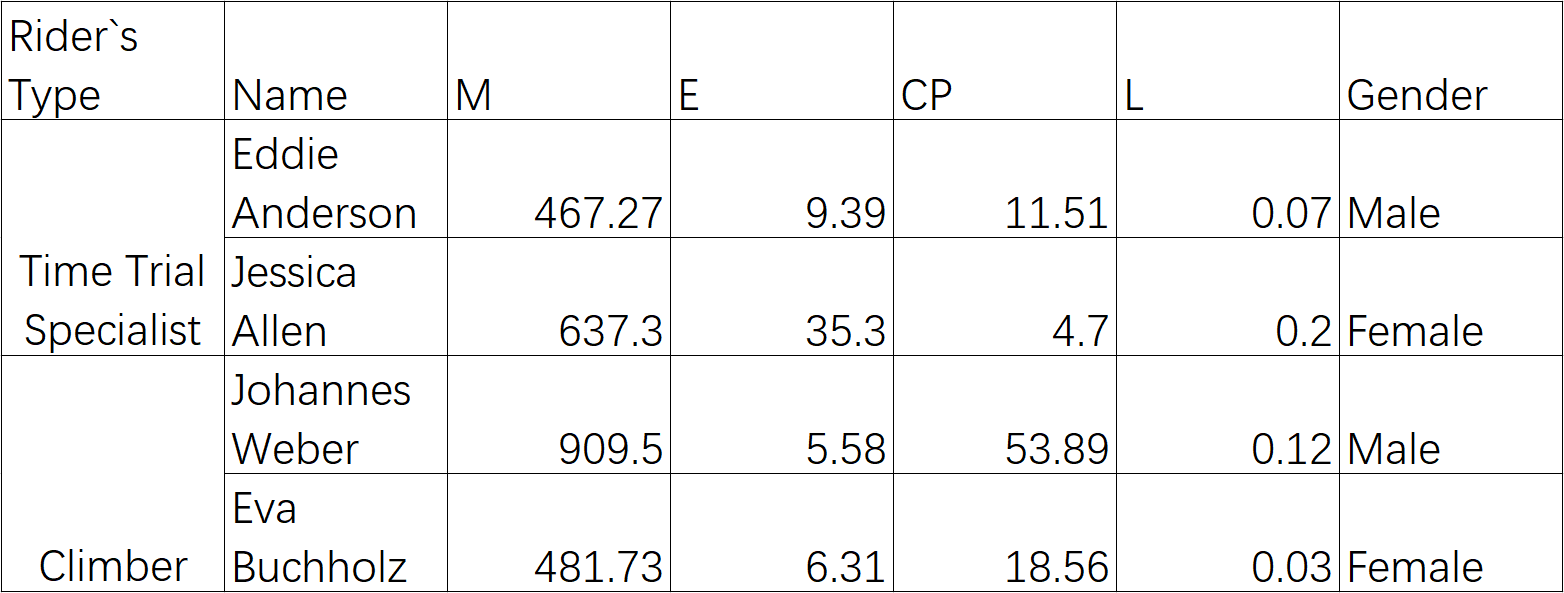
\includegraphics[width=.8\columnwidth]{Rider's profile.jpg}
    \caption{Rider's profile}
\end{figure}
According to the profile, the climbers has a faster recover rate, this match the common view. Climbers also have a great ability to recover between efforts they make on
the mountain. This means that they can go into an anaerobic effort such as an attack and recover from it quickly in order to make another acceleration.

The TT specialist, in the other hand has a higher Stamina-to-work conversion efficiency, which helps them to sustain a higher power for a longer time, it is a great advantage
in a TT race.

\section{Requirement 2: Test}
Here we will apply our model to a time trial courses--the 2021 UCI World Championship time trial course in Flanders, Belgium --for each power profile we defined
above to prove that out model can be solved, the value of some parameter is show below:
\begin{table}[H]
    \centering
    \begin{tabular}{cc}
        \toprule
        \bf Parameters & \bf Values \\
        \midrule
        $C_r$          & 0.003      \\
        $m$            & 80         \\
        $g$            & 9.8        \\
        $\eta $        & 0.95       \\
        $\rho  $       & 1.2        \\
        $c_wA$         & 0.31       \\
        \bottomrule
    \end{tabular}
    \caption{Value of some parameters, from https://www.sheldonbrown.com/rinard/aero/formulas.html}
\end{table}
We first find the course profile -- the route map and the topographic map of the course (from https://www.flanders2021.com)
then use the Reverse-Engineering Visualizations method developed by Jorge Poco1 and Jeffrey Heer in 2017\cite{poco2017reverse} to get the data we need about the racing track,
which is two two-dimensional matrices, we plot the two matrix to demonstrate them.

\begin{figure}[H]
    \centering
    \subcaptionbox{Men elite route map}{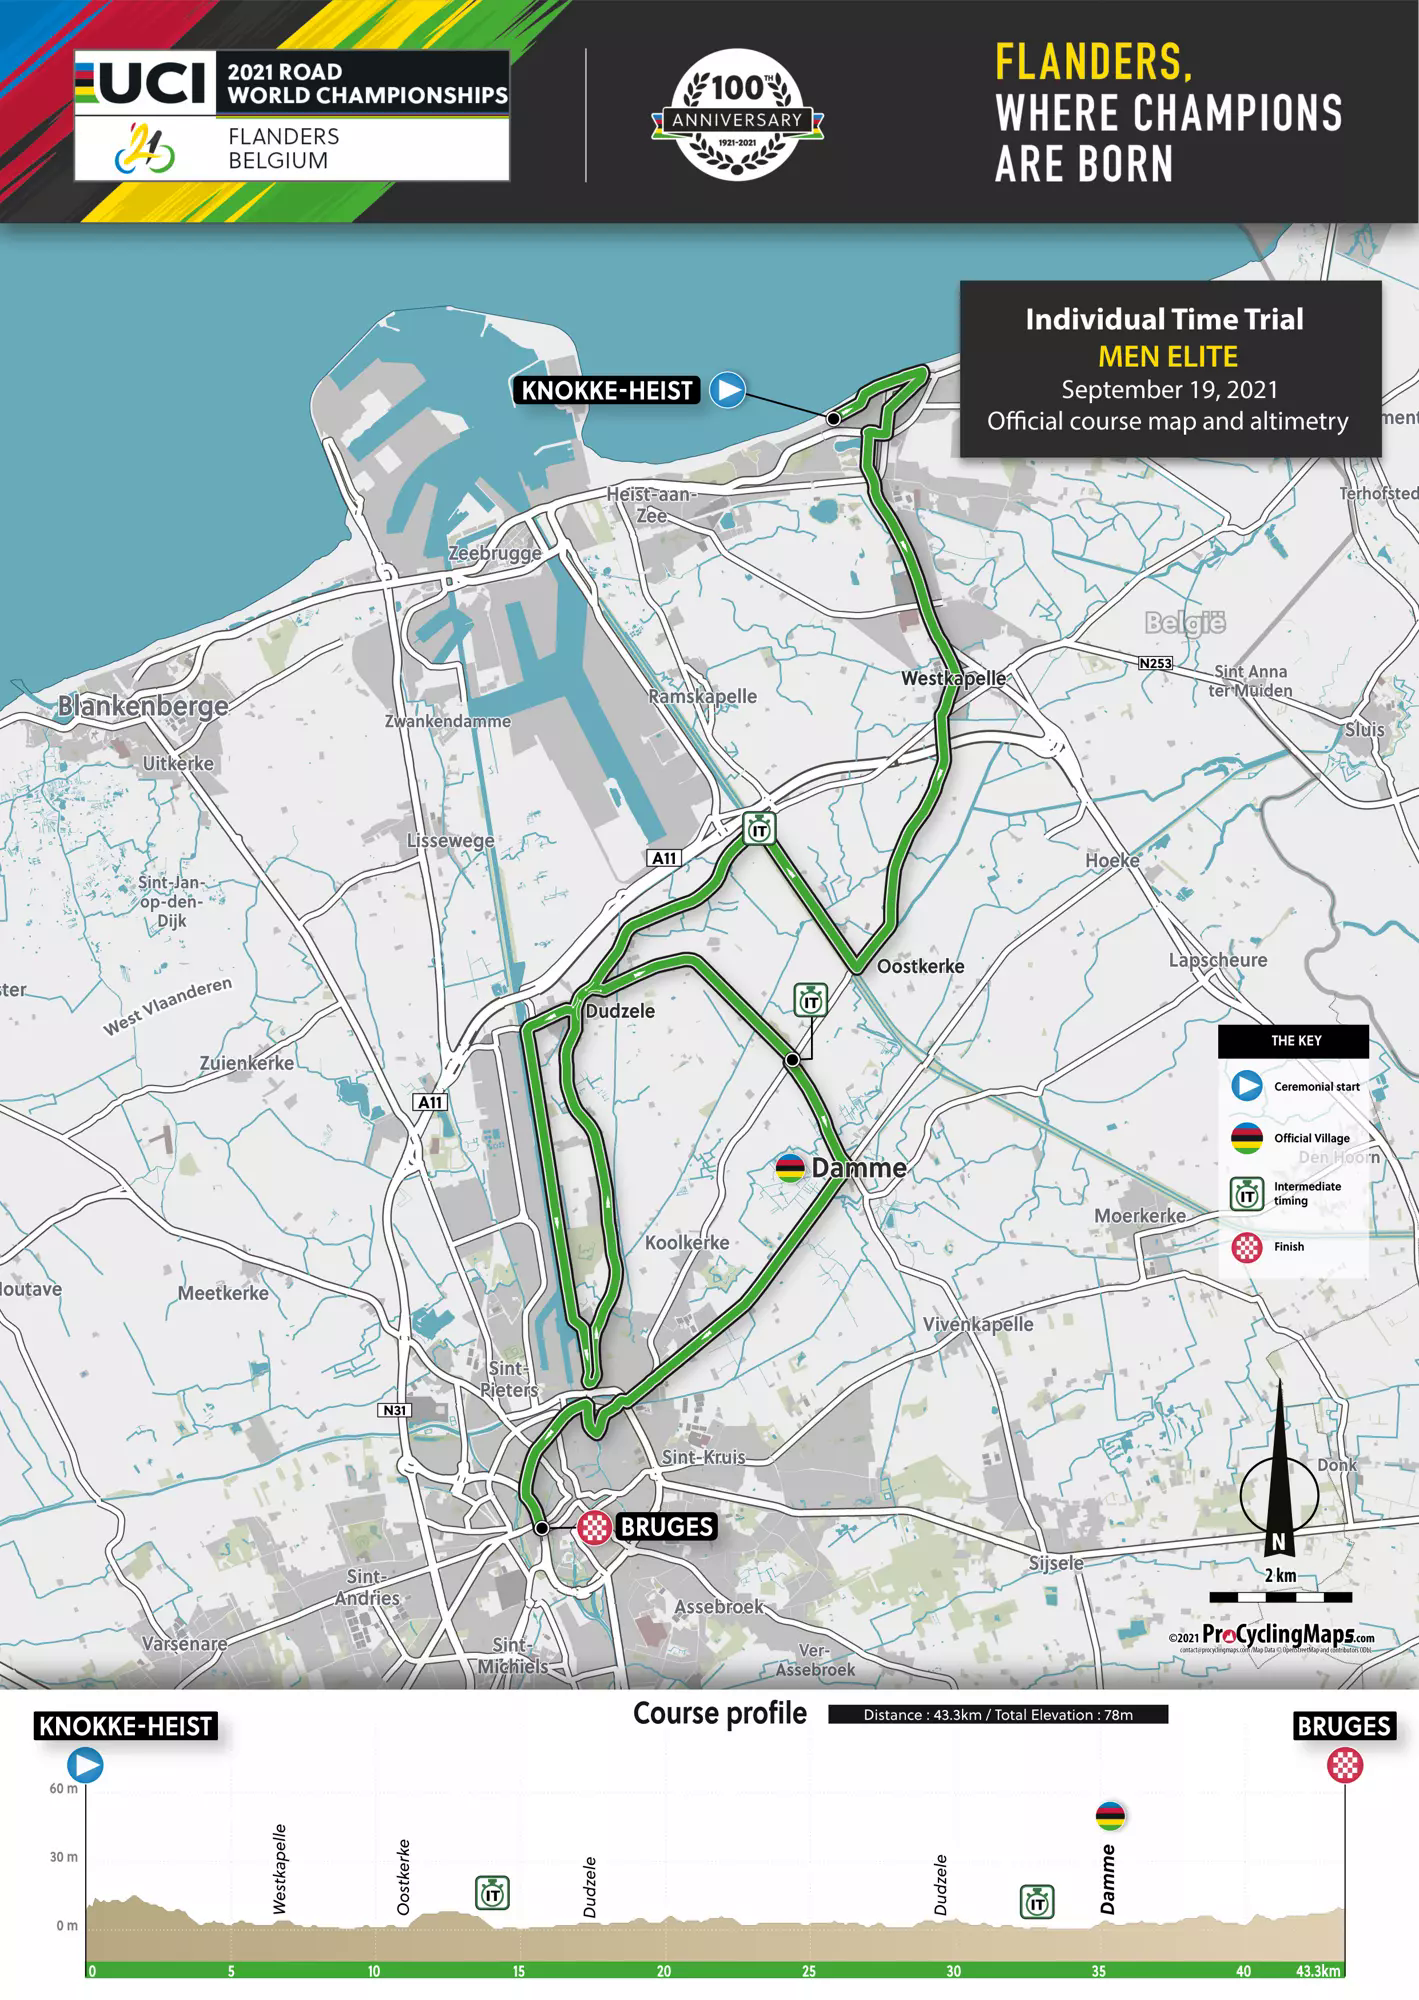
\includegraphics[width=0.4\columnwidth]{men-elite-individual-time-trial-map}}
    \subcaptionbox{Men elite route map matrix demo}{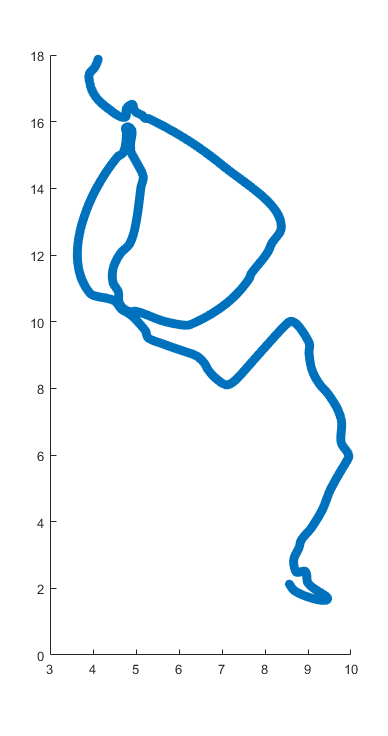
\includegraphics[width=0.4\columnwidth]{man_elite_map_matrix_demo}}

    \subcaptionbox{Men elite topographic map}{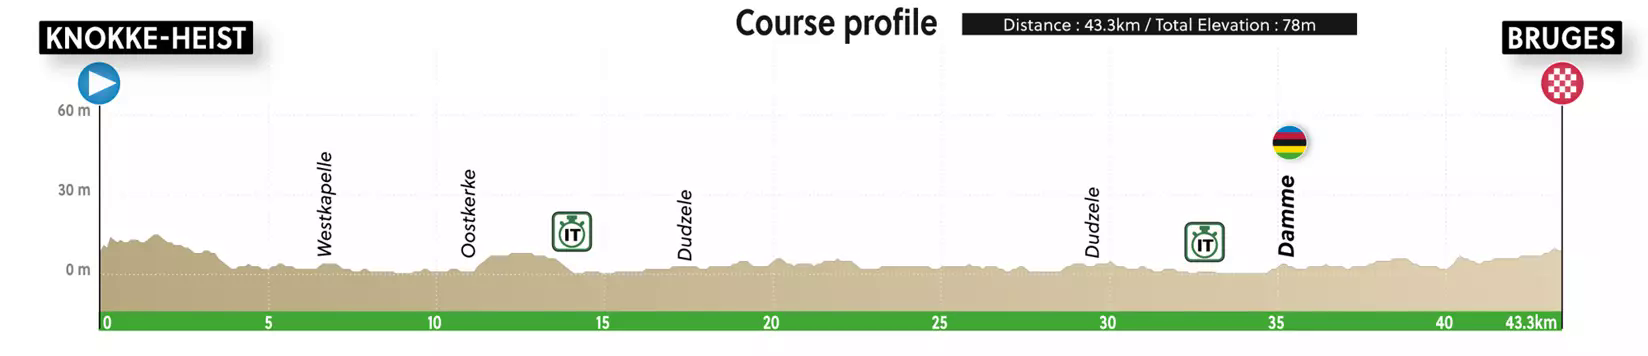
\includegraphics[width=1\columnwidth]{men-elite-individual-time-trial-profile}}

    \subcaptionbox{Men elite topographic map matrix demo}{
\includegraphics[width=1\columnwidth]{men-elite-individual-time-trial-profile-matrix demo}}
    \caption{Course's map}
\end{figure}


\begin{figure}[H]
    \centering
    \subcaptionbox{Eddie Anderson's power curve}{\includesvg[width=.4\columnwidth]{"csi4"}}
    \subcaptionbox{Jessica Allen's power curve}{\includesvg[width=.4\columnwidth]{"csi3"}}

    \subcaptionbox{Johannes Weber's power curve}{\includesvg[width=.4\columnwidth]{"csi2"}}
    \subcaptionbox{Eva Buchholz's power curve}{\includesvg[width=.4\columnwidth]{"csi1"}}
    \caption {power curves of the chosen riders}
\end{figure}

\begin{figure}[H]
    \centering
    \subcaptionbox{Self designed route map matrix demo}{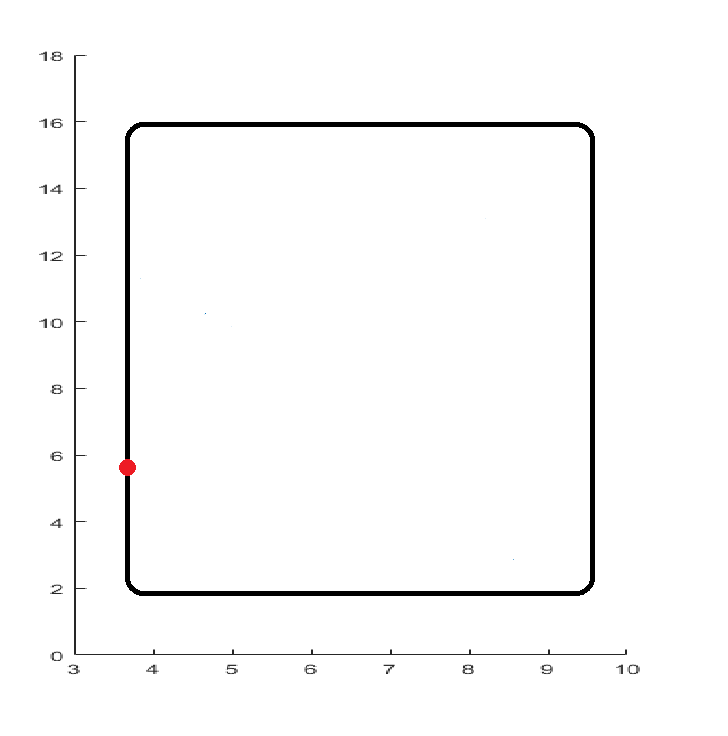
\includegraphics[width=.4\columnwidth]{self-designed_map_matrix_demo}}
    \subcaptionbox{Self designed topographic map matrix demo}{\includesvg[width=.4\columnwidth]{triangle}}
    \caption{Self-designed map}
\end{figure}
\begin{figure}
    \centering
    \includesvg[width=.6\columnwidth]{"squ3s15"}
    \caption{Jessica Allen's power curve in the self-designed map}
\end{figure}
After a few tests, we find the best power curve for each of the four riders, in the tests, we realized that
our model has the following advantages:
\begin{enumerate}
    \item We discretized the race, thus we are able to use the dynamic programming method, which make sure we find the global optimal solution %应用了动态规划,能保证得到全局最优解
    \item We improved our computing efficiency.%计算效率高
    \item The model of P-D relationship is supported by multiple articles and the fitting is almost perfect.
    \item The solution provided by the model is very effective, it greatly cut the time the riders need to finish the race.
    \item The model can be applied to any type of battery of the same battery type.
\end{enumerate}
However, there are also some disadvantages that we can not ignore:
\begin{enumerate}
    \item The influence between the riders were not taken into account, in a real race the rider will try to grab a vantage point, which may force some riders to
          slow down. What's more, they will disrupt the airflow, which will change the air friction.%忽略了运动员之间的影响
    \item We didn't consider that the models of movement will be different from the one on the straight road, in our model, the rider was like riding on a straight path
          all the time.%规划策略可能不易实行
    \item Even though we have discretized the race, our model' instructions are still too ideal, the riders will still have to change their power constantly, which is
          almost impossible in any race. %没有考虑转弯
\end{enumerate}
\section{Requirement 3}
In the first two requirements, the speed of wind($v_m$) is always zero, and it will result in a decrease in simulation accuracy.
Now we take the influence of the wind into account,  $v_m$, which means the speed of wind, will be given a constant value, but its direction will change, the
to test the sensitivity of the model, if the change of the time needed to finish the race will not vary significantly the sensitivity of our model
is considered low, after another few tests, the result is shown below.
\begin{figure}
    \centering
    \includesvg[width=1\columnwidth]{"radar"}
    \caption{Sensitive analysis}
\end{figure}
When the wind speed is set at 10$m/s$ the influence is relatively small-the maximum difference is just over 100s, which is negligible when compare to the total time of
near an hour. The result is thrilling, for it means that our model is not very sensitive to the change of the weather, windy or not, the model tends to give similar--and
equally useful--guidance. Which means we don't have to predict the future weather when we try to find the best solution for the race, and it makes to model more trustworthy.
\section{Requirement 4}
As mentioned before, the guidance given by our current model is too detailed and ideal, thus we are concerned that whether the model will be impractical if the rider can't
follow the instructions. In this section, we will try to find a way to simulate the influence of missing the power target. Here we will use the sliding window algorithm which
has a window of 7, meaning that the value of the note will be reassigned to the mean value of three values on both sides and itself. This algorithm will make the curve smooth, which is closer to reality.
\begin{figure}
    \centering
    \includesvg[width=1\columnwidth]{"smoothed"}
    \caption{Smooth power curve}
\end{figure}
\section{Requirement 5}
Again we will try to improve our model, this time we will analyze the proper way of team work. The extended new model should be able to  include the optimal power use for a team time trial of six riders per team, where the team's time is
determined when the fourth rider crosses the finish line. Clearly, the two slowest member matter little, what's important is how the first three riders should help the forth.

To find a way to analyze the influence of the teammates, we need a model of the windbreakers, which described how the air friction will change according to the relative
position of the team members.
\newpage
\section{Requirement 6}
\begin{center}
    \huge \textbf{Rider's Guidance}
\end{center}\large
You have been training and focussing on this race for a while; you  have just progressed from youth races to your first junior race; you are experienced in riding.
However, taking part in the race on the open road in a bunch is an exciting challenge, and you don't want to make any mistakes.
Understanding the techniques, skills, etiquette and rules will help keep the race safe and enjoyable for everyone. Now I must ask all of you to pay close attention to the instructions in the guide and use your power meter
to help you control your pace to meet its required so that you can make the best of yourself without hurting yourself with the high tensity of the race and your eager for
the champion. This knowledge can also significantly improve your chances of finishing in the best possible place in the results!

Time trials are called the 'race of truth' for good reason. There's no hiding in the bunch before the sprint, you have to work for your speed every inch of the way, so it
became extremely  important to keep a reasonable pace, and this guidance aims to help you do so.
Recently a new model has been developed to find the best racing strategy for each rider, from your trainings and races in the past, it was able to quantificate your ability
like stamina, recovery, critical power and maximum power the model will show you when to slow down and when to speed up, with a proper pace you will be able to ride
fast and easy.

So here are the general suggestion of the model:
\begin{enumerate}
    \item Always keeps a steady pace, in the %%%%%%%%%%%%%%%%%%%%%%%%%%%%%%%%%%%%%%%%%
\end{enumerate}

A pre-performance routine means your attention stays in the present and only on elements that are task-relevant. It helps reduce anxiety, gets you to your optimal level
of nerves, and improves concentration, focus and performance.

The routine gets you ready to compete, feeling comfortable you have done everything possible to reach the start line with the best preparation. The more you repeat and
practice the routine, the more beneficial it is. I hope you have all remembered the instructions above, and it is ok if you didn't, you will remember them in a few routines.
Now go!


\bibliographystyle{plain}
\bibliography{2022_MCM_ICM_Report}
%%%%%%%%%%% End Paper %%%%%%%%%%%
\end{document}
\end
